\documentclass[a4paper,12pt,spanish]{article}
\usepackage[spanish,activeacute]{babel}
\usepackage[utf8]{inputenc}
\usepackage{tocbibind}
\usepackage[colorlinks=true,linkcolor=blue]{hyperref}
\usepackage{eurosym}
\usepackage{listings}
\usepackage{color}
\usepackage{fancyvrb}
\usepackage{times}
\usepackage{sans}

\definecolor{gray97}{gray}{.95}
\definecolor{gray75}{gray}{.75}
\definecolor{gray45}{gray}{.45}

\lstset{ frame=Ltb,
     framerule=0pt,
     aboveskip=0.5cm,
     framextopmargin=3pt,
     framexbottommargin=3pt,
     framexleftmargin=0.4cm,
     framesep=0pt,
     rulesep=.4pt,
     backgroundcolor=\color{gray97},
     rulesepcolor=\color{black},
     %
     stringstyle=\ttfamily,
     showstringspaces = false,
     basicstyle=\small\ttfamily,
     commentstyle=\color{gray45},
     keywordstyle=\bfseries,
     %
     numbers=left,
     numbersep=15pt,
     numberstyle=\tiny,
     numberfirstline = false,
     breaklines=true,
   }

% minimizar fragmentado de listados
\lstnewenvironment{listing}[1][]
   {\lstset{#1}\pagebreak[0]}{\pagebreak[0]}

\lstdefinestyle{consola}
   {basicstyle=\scriptsize\bf\ttfamily,
    backgroundcolor=\color{gray75},
   }
 
\lstdefinestyle{Java}
   {language=Java,
   }

\RequirePackage{ifpdf} % ¿latex o pdflatex?
% Configuración de las imágenes
\ifpdf
	\usepackage[pdftex]{graphicx}	% Inclusión de imágenes
	\DeclareGraphicsExtensions{.pdf,.png,.jpg}
\else
	\usepackage{graphicx}		% Inclusión de imágenes
	\DeclareGraphicsExtensions{.eps}
\fi
\graphicspath{ {./img/} } % Ruta respecto al fichero tex principal dónde se buscan

\oddsidemargin 0in
\textwidth 6.5in
\topmargin -0.5in
\textheight 9.5in
\parindent 0em

\author{Adrián Cepillo Macías}
\title{Tutorial de Eclipse \\SpringSource Tool Suite}

\begin{document}
\begin{titlepage}
  \maketitle
  \begin{figure}[h!]
    \centering
    
\includegraphics[scale=0.75]{sts}
    \label{fig:Portada}
  \end{figure}
\end{titlepage}
 
\tableofcontents
\newpage 

\section{Instalación de Eclipse SpringSource Tool Suite}

El software que se va usar durante el curso es una versión de eclipse preparada para trabajar con spring, grails y groovy. A continuación se explicará desde donde descargarlo y como instalarlo.

\subsection{Descarga}

Puede descargar la aplicación desde el siguiente enlace a \href{http://www.springsource.com/products/springsource-google-download?utm\_source=eclipse.org\&utm\_medium=web\&utm\_content=promotedDL\&utm\_campaign=STS}{Spring Tool Suite}.

\begin{center}
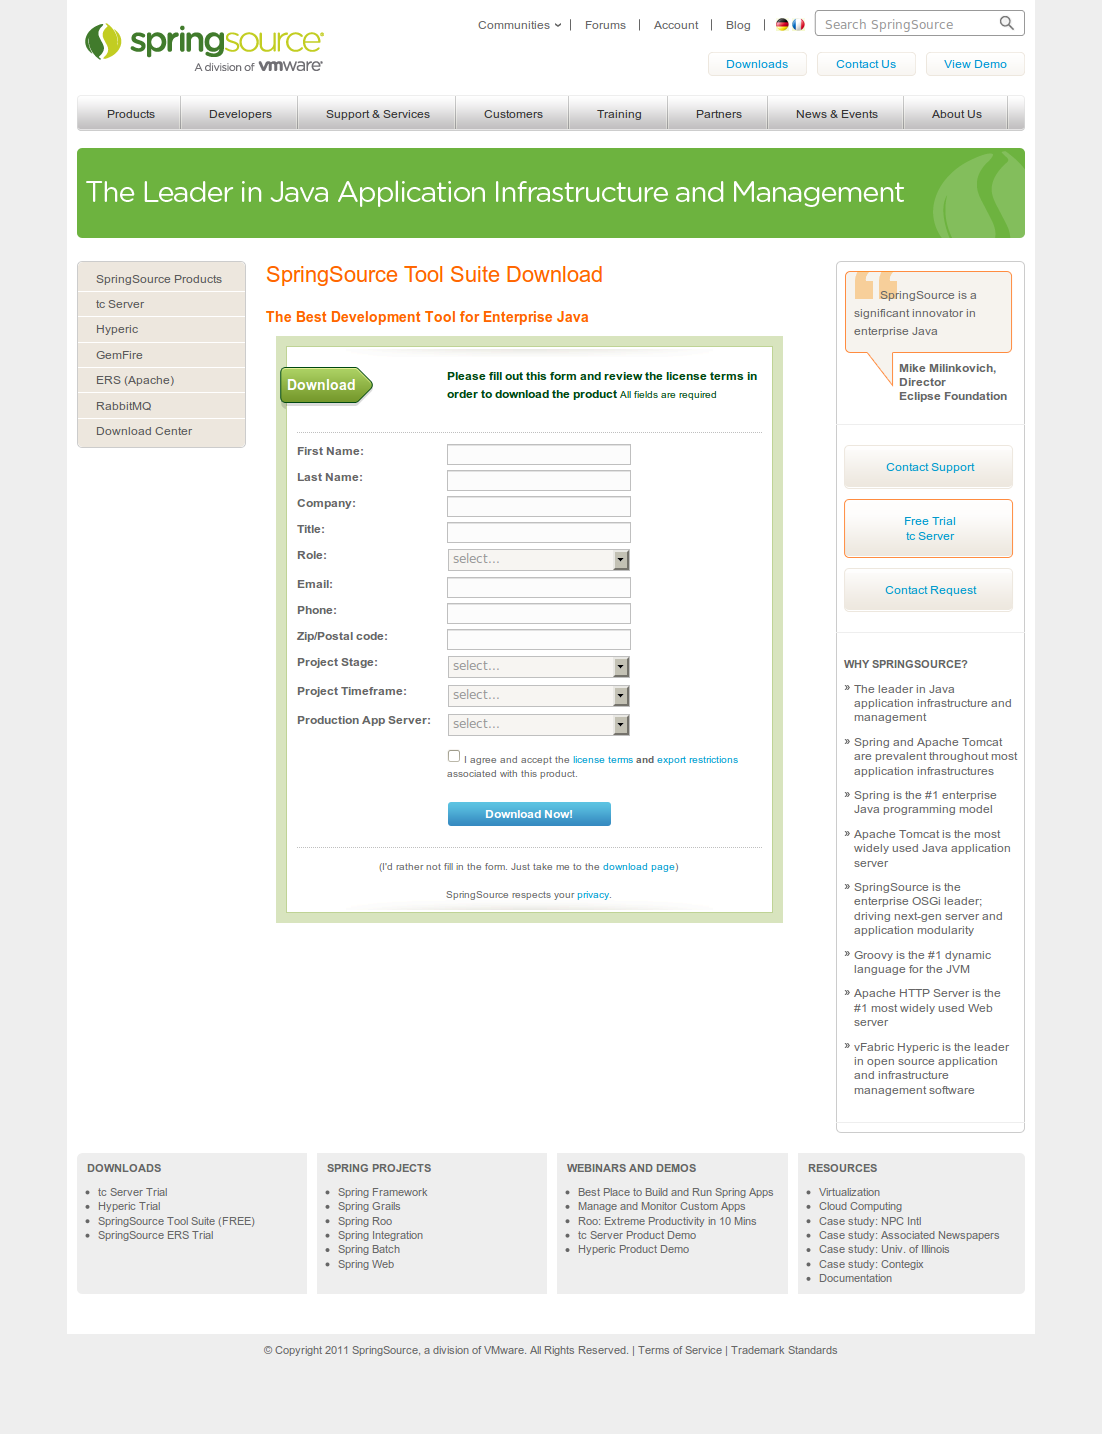
\includegraphics[scale=0.35]{SpringSourceToolSuiteDownload}
\end{center}

\subsection{Instalación}

Tras haber descargado la aplicación habrá un terminal he introduzca el siguente comando:

\begin{itemize}
\item \$ sh springsource-tool-suite-2.7.1.RELEASE-e3.7-linux-gtk-x86\_64-installer
\end{itemize}

Se abrirá el interfaz gráfico de la aplicación. 
Haga click en next y siga las intrucciones. 

\begin{center}
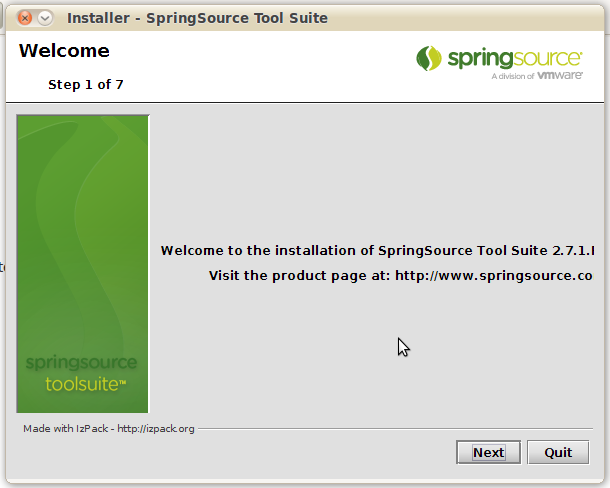
\includegraphics[scale=0.5]{ide}
\end{center}

Acepte la licencia y continúe.

\begin{center}
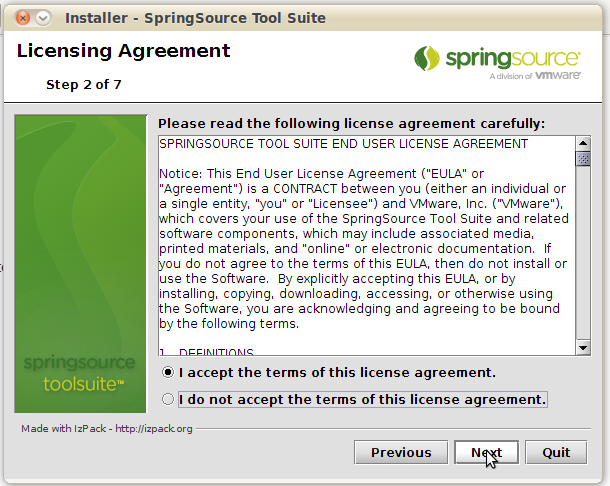
\includegraphics[scale=0.5]{ide2}
\end{center}

Elija el directorio dónde se instalará la aplicación.

\begin{center}
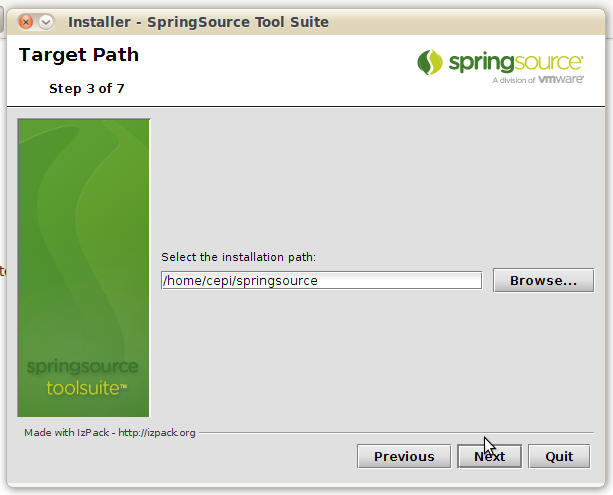
\includegraphics[scale=0.5]{ide3}
\end{center}

Seleccione las todas la opciones a instalar.

\begin{center}
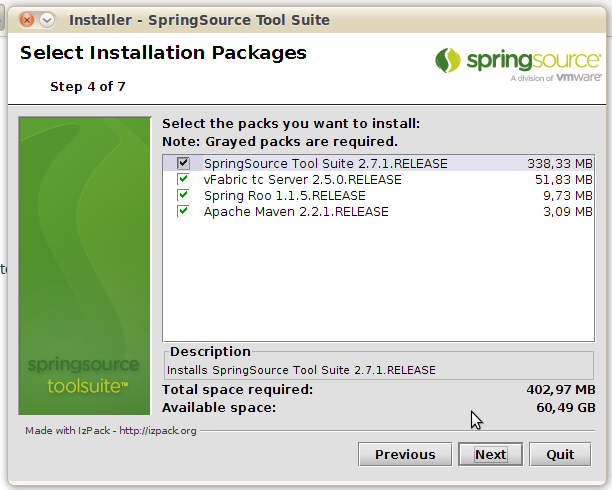
\includegraphics[scale=0.5]{ide4}
\end{center}

Ahora elija la carpeta donde se encuentre Java JDK. Puede descargar la última versión \href{http://download.oracle.com/javase/7/docs/webnotes/install/linux/linux-jdk.html}{aquí}. En esa misma web puede encontrar las instrucciones apra su instalación.

\begin{center}
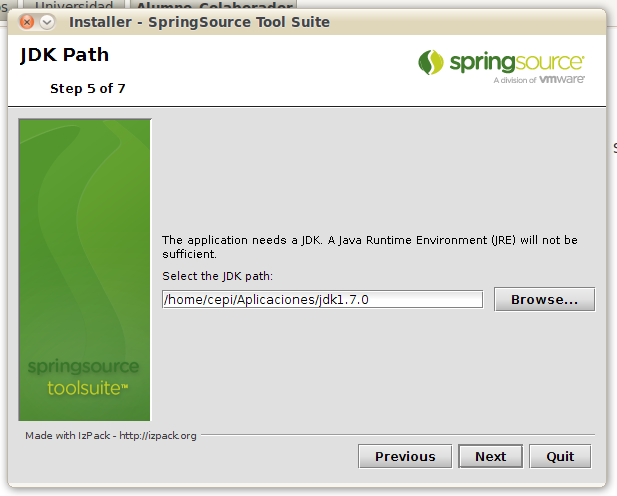
\includegraphics[scale=0.5]{ide5}
\end{center}

Un último Next y la aplicación se instalará.

\begin{center}
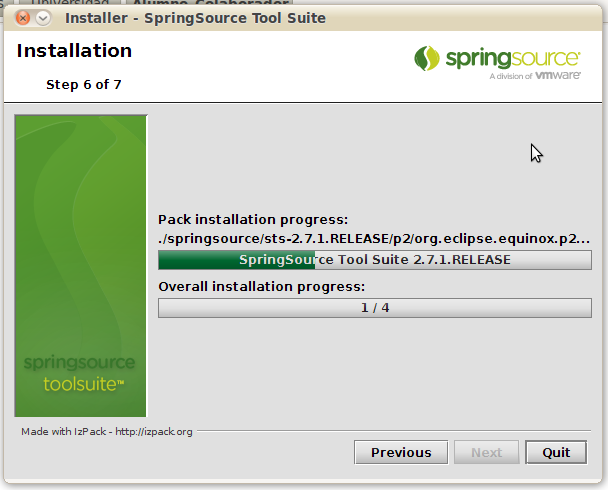
\includegraphics[scale=0.5]{ide6}
\end{center}

\section{Empezar a trabajar con Eclipse}

Vamos a la carpeta donde hemos instalado Eclipse STS y ejecutamos el fichero {\it STS}. La aplicación tardará un poco en abrirse, si no es así, se ha de comprobar los permisos de lectura y ejecución de este mismo.\\

Una vez abierto debemos clickar en {\it extensions}. Marcamos {\it Grails}, más abajo {\it Grails Support} y {\it Groovy Eclipse}. Pulsamos instalar y aceptamos las licencias.

\begin{center}
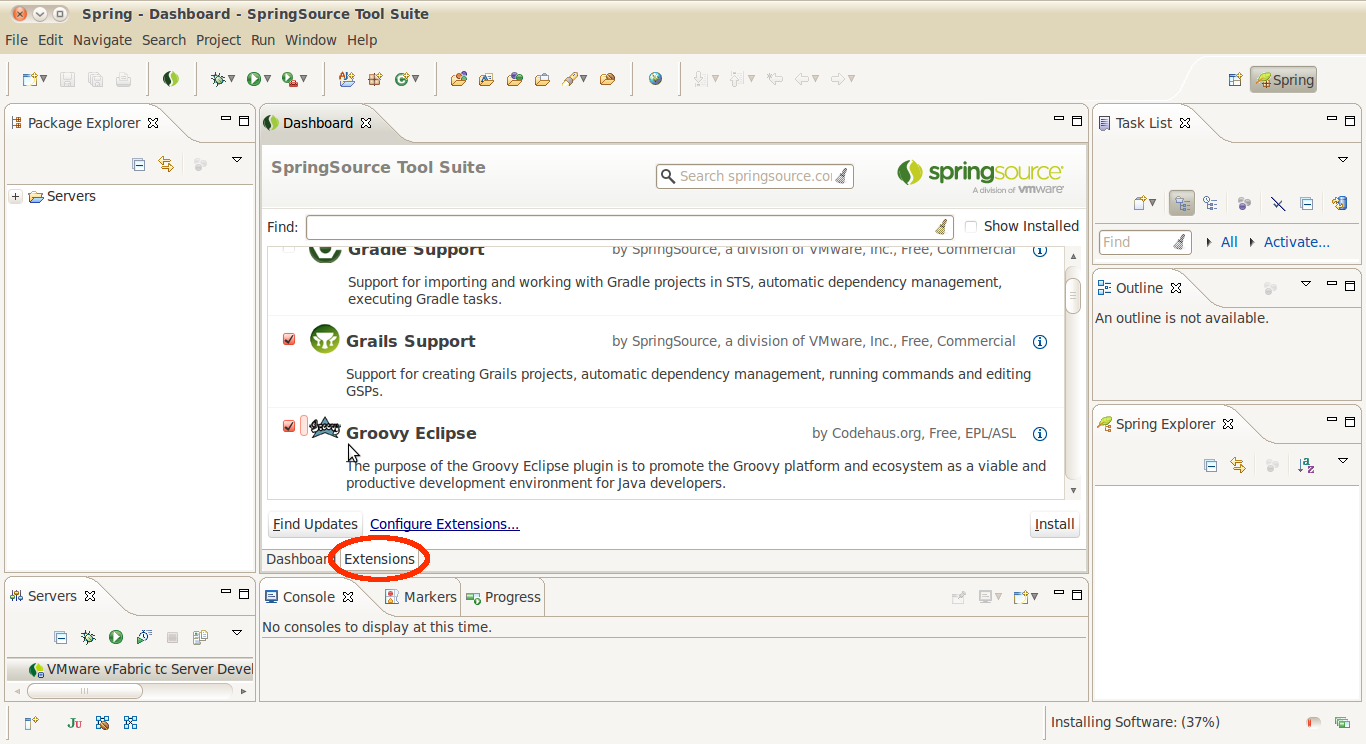
\includegraphics[scale=0.35]{ide9}
\end{center}

Habrá que reiniciar Eclipse STS para notar los cambios. Una vez abierta de nuevo la aplicación, pichamos en File-$>$New-$>$Grails Project para generar la estructura básica de grails.\\ 

{\bf Nota:} Aparecerá un ventana avisando del cambio de vista al crear un proyecto Grails. Aceptamos. Podemos cerrar las ventanas que no sean útiles dejando solo la consola, el código y el explorador del proyecto a la izquierda.

\begin{center}
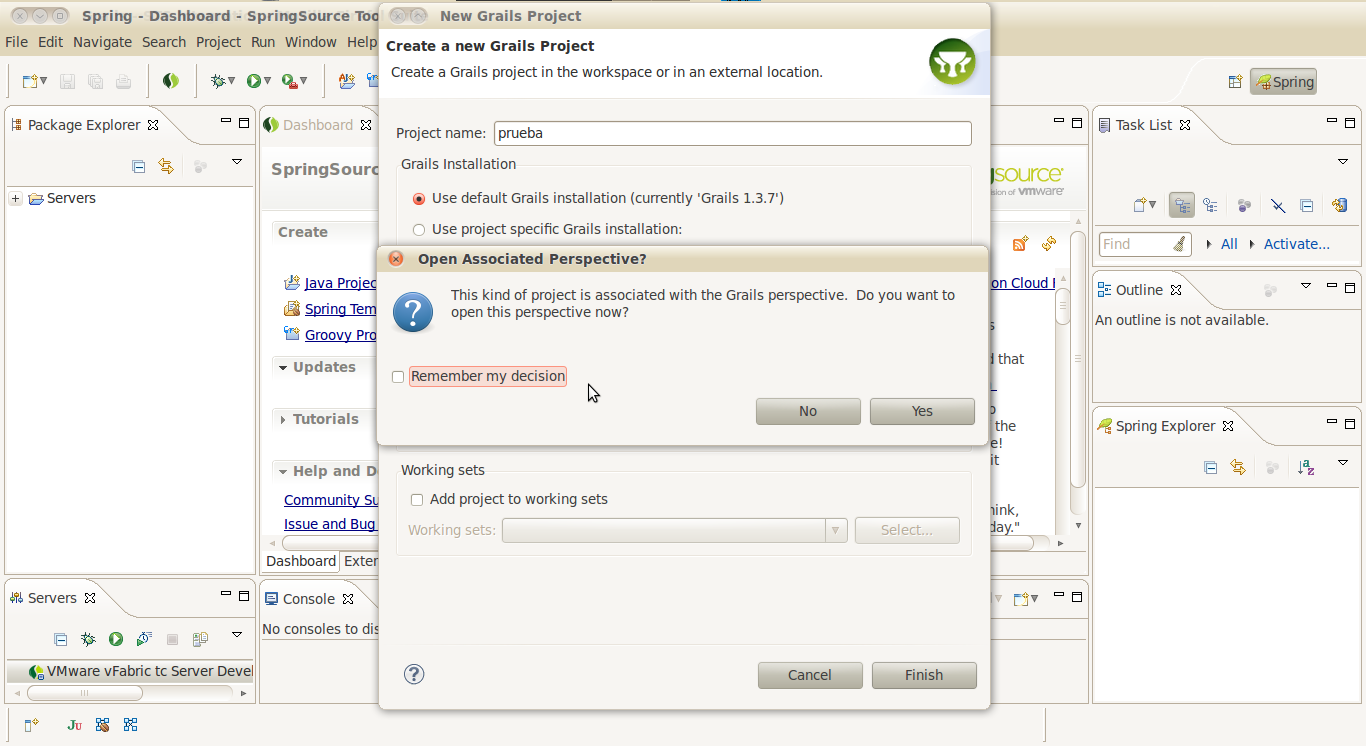
\includegraphics[scale=0.35]{ide10}
\end{center}

\section{Un pequeño ejemplo con Grails}

Después de haber creado el proyecto, vamos a hacer una pequeña aplicación donde podremos crear, editar y eliminar libros y luego visualizarlos. Para ello solo tenemos que crear un controlador y un dominio de modelo.

\subsection{Domain Class: Book}

Primero vamos con la clase de dominio llamada {\it Book}. Nos vamos a la jerarquía del proyecto, hacemos click con el botón derecho en {\it domain class}, luego New-$>$Domain Class. E introducimos como nombre {\it org.example.Book}. Grails creará el paquete {\it org.example}, el cuál contendrá el fichero {\it Book.groovy}. La ruta donde se encuentra este archivo será {\it wokspace-sts-2.7.1.RELEASE/mi-proyecto/grails-app/domain/org/example/Book.groovy}.\\

Realiza las modificaciones pertinentes a la plantilla de inicio según el siguiente código:

\lstinputlisting[style=Java]{resources/Book.groovy}

\subsection{Controller Class: BookController}

Hacemos los mismo para Controller. Y le ponemos el mismo nombre {\it org.example.Book}, el fichero se llamará {\it BookController.groovy}.
Definimos el scaffolding para la clase Book.

\lstinputlisting[style=Java]{resources/BookController.groovy}

\section{Correr la aplicación con Eclipse}

Una vez hecho esto pinchamos en Run As-$>$1. Grails Command (run-app). Se abrirá la consola de Eclipse, grails generará la aplicación y se iniciará el servidor, finalmente se mostrará una url para visualizar la aplicación, podemos copiarla en nuestro navegador favorito o clickar y verlo en el navegador de Eclipse.

\end{document}